\section{Adresiranje}
IP adresa je adresa koja ima informacije o tome kako do\'{c}i do određenog hosta, posebno van LAN-a. IP adresa je 32-bitna jedinstvena adresa koja ima adresni prostor od $2^{32}$. Generalno, postoje dve notacije u kojima je IP adresa zapisana, tačkasta decimalna notacija i heksadecimalna notacija.

\begin{figure}[H]
    \centering
    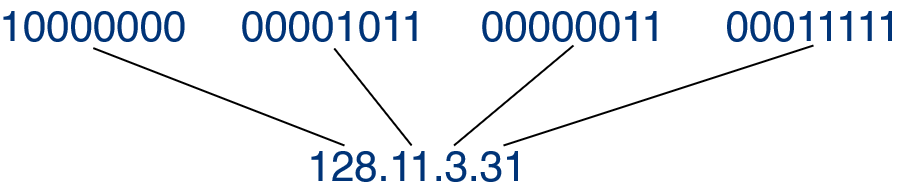
\includegraphics[width=0.75\textwidth]{Slike/Tackasta notacija.png}
    \caption{Tačkasta decimalna notacija}
    \label{fig:ip_adresiranje}
\end{figure}

\begin{figure}[H]
    \centering
    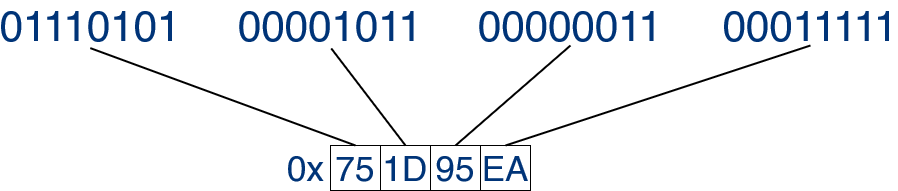
\includegraphics[width=0.75\textwidth]{Slike/Heksadecimalna notacija.png}
    \caption{Heksadecimalna notacija}
    \label{fig:heksadecimalna_notacija}
\end{figure}

\subsubsection{Klase}

Klase IP adrese se koriste za određivanje bitova koji se koriste za ID mreže i ID hosta i broj ukupnih mreža i hostova mogu\'{c}ih u toj određenoj klasi. Svaki ISP ili administrator mreže dodeljuje IP adresu svakom uređaju koji je povezan na njegovu mrežu. 32-bitna IP adresa je podeljena u pet podklasa koje se mogu videti u tabeli \ref{tab:klase_namene}. Određivanje mrežnih bitova je prikazano u tabeli \ref{tab:klase_opsezi}.\\

\begin{table}[]
    \begin{center}
    \begin{tabular}{lc}
    Klasa & Namena              \\ \hline\hline
    A     & Velike mreže        \\
    B     & Srednje mreže       \\
    C     & Male mreže          \\
    D     & Multicast           \\
    E     & Naučno-Istraživačke
    \end{tabular}
    \caption{Klase i njihove namene}
    \label{tab:klase_namene}
    \end{center}
\end{table}



\begin{table}[]
    \begin{center}
    \begin{tabular}{lc|cccc}
    Klasa & Opseg     & \multicolumn{1}{c|}{1. bajt} & \multicolumn{1}{c|}{2. bajt} & \multicolumn{1}{c|}{3. bajt} & 4. bajt \\ \hline\hline
    A     & 0 - 126   & \multicolumn{1}{c|}{Mrežni}  & \multicolumn{1}{c|}{Host}    & \multicolumn{1}{c|}{Host}    & Host    \\
    B     & 128 - 191 & \multicolumn{1}{c|}{Mrežni}  & \multicolumn{1}{c|}{Mrežni}  & \multicolumn{1}{c|}{Host}    & Host    \\
    C     & 192 - 223 & \multicolumn{1}{c|}{Mrežni}  & \multicolumn{1}{c|}{Mrežni}  & \multicolumn{1}{c|}{Mrežni}  & Host    \\ \cline{3-6} 
    D     & 224 - 239 & \multicolumn{4}{c}{\multirow{2}{*}{Nema podmrežnu masku}}                                            \\
    E     & 240 - 255 & \multicolumn{4}{c}{}                                                                             
    \end{tabular}
    \caption{Opsezi i bajtovi podmaski}
    \label{tab:klase_opsezi}
    \end{center}
\end{table}

\textbf{Posebne adrese: }
\emph{Lokalne adrese veza:} 169.254.0.0 – 169.254.0.16
\emph{Povratne adrese:} 127.0.0.0 – 127.255.255.255
\emph{Komunikacija unutar trenutne mreže:} 0.0.0.0 – 0.0.0.8

\subsubsection{Pravila za dodeljivanje ID mreže}
Hostovi koji se nalaze na istoj fizičkoj mreži se identifikuju po ID-u mreže, pošto je svim hostovima na istoj fizičkoj mreži dodeljen isti mrežni ID. ID mreže se dodeljuje na osnovu slede\'{c}ih pravila:
\begin{itemize}
    \item Mrežni ID ne može da počinje sa 127 jer je 127 rezervisan za interne funkcije povratne petlje.
    \item Svi bitovi mrežnog ID-a postavljeni na 0 koriste se za označavanje određenog hosta na lokalnoj mreži i ne rutiraju se i stoga se ne koriste.
    \item Svi bitovi mrežnog ID-a postavljeni na 255 rezervisani su za koriš\'{c}enje kao IP adresa emitovanja i stoga se ne mogu koristiti.
\end{itemize}

\subsubsection{Pravila za postavljanje ID hosta}
ID-ovi hosta se koriste za identifikaciju hosta unutar mreže. ID hosta se dodeljuje na osnovu slede\'{c}ih pravila:\\
\begin{itemize}
    \item Unutar bilo koje mreže, ID hosta mora biti jedinstven za tu mrežu.
    \item ID hosta u kome su svi bitovi postavljeni na 0 ne može se dodeliti jer se ovaj ID hosta koristi za predstavljanje mrežnog ID-a IP adrese.
    \item ID hosta u kome su svi bitovi postavljeni na 255 ne može se dodeliti jer je ovaj ID hosta rezervisan kao adresa za emitovanje za slanje paketa svim hostovima prisutnim na toj određenoj mreži.
\end{itemize}
